\documentclass{beamer}
%
% Choose how your presentation looks.
%
% For more themes, color themes and font themes, see:
% http://deic.uab.es/~iblanes/beamer_gallery/index_by_theme.html
%
\mode<presentation>
{
  \usetheme{default}      % or try Darmstadt, Madrid, Warsaw, ...
  \usecolortheme{spruce} % or try albatross, beaver, crane, ...
  \usefonttheme{default}  % or try serif, structurebold, ...
  \setbeamertemplate{navigation symbols}{}
  \setbeamertemplate{caption}[numbered]
} 

\usepackage[english]{babel}
\usepackage[utf8x]{inputenc}
\usepackage[absolute,overlay]{textpos}

\title[Blender Intro]{Blender intro}
\author{Łukasz Hryniuk}
\date{October 25, 2018}

\begin{document}

\begin{frame}
  \titlepage
  \centering\href{https://github.com/hryniuk/blender-intro}{github.com/hryniuk/blender-intro}
\end{frame}

\begin{frame}
\begin{figure}
	
\includegraphics[keepaspectratio,height=9cm]{blender-intro.png}
\end{figure}
\end{frame}

\begin{frame}{Outline}
  \tableofcontents
\end{frame}

\section{Introduction}

\begin{frame}{About me and you}

\begin{itemize}
\item About me
	\begin{itemize}
		\item \textbf{Digital art hobbyist (Blender\&Krita)}
		\item Software Developer (at Sperasoft)
		\item Free and Open Source Enthusiast
	\end{itemize}
\item About you
	\begin{itemize}
		\item Do you draw?
		\item Do you use computer to create art?
		\item Do you use Blender?
		\item Do you plan to use Blender after this talk?
	\end{itemize}
\end{itemize}

\end{frame}

\begin{frame}{Motto}

\centering \Huge
\emph{Blender is not so hard to learn and worth trying}

\end{frame}

\begin{frame}{What's Blender}

\begin{itemize}
  \item free and open source 3D creation suite
  \item \textbf{allows Python scripting}
  \item video editor (nice example: rotoscoping)
  \item 2d  animation suite (to be improved in Blender 2.8)
  \item includes Blender Game Engine
\end{itemize}

\end{frame}

\begin{frame}{Possibilities}

Open movies:
\begin{itemize}
	\item Agent 327: Operation Barbershop (2017) - “the Netherlands’ answer to 
	James Bond"
	\item Cosmos Laundromat (2015)
	\item Big Buck Bunny (2008)
\end{itemize}

\begin{figure}
	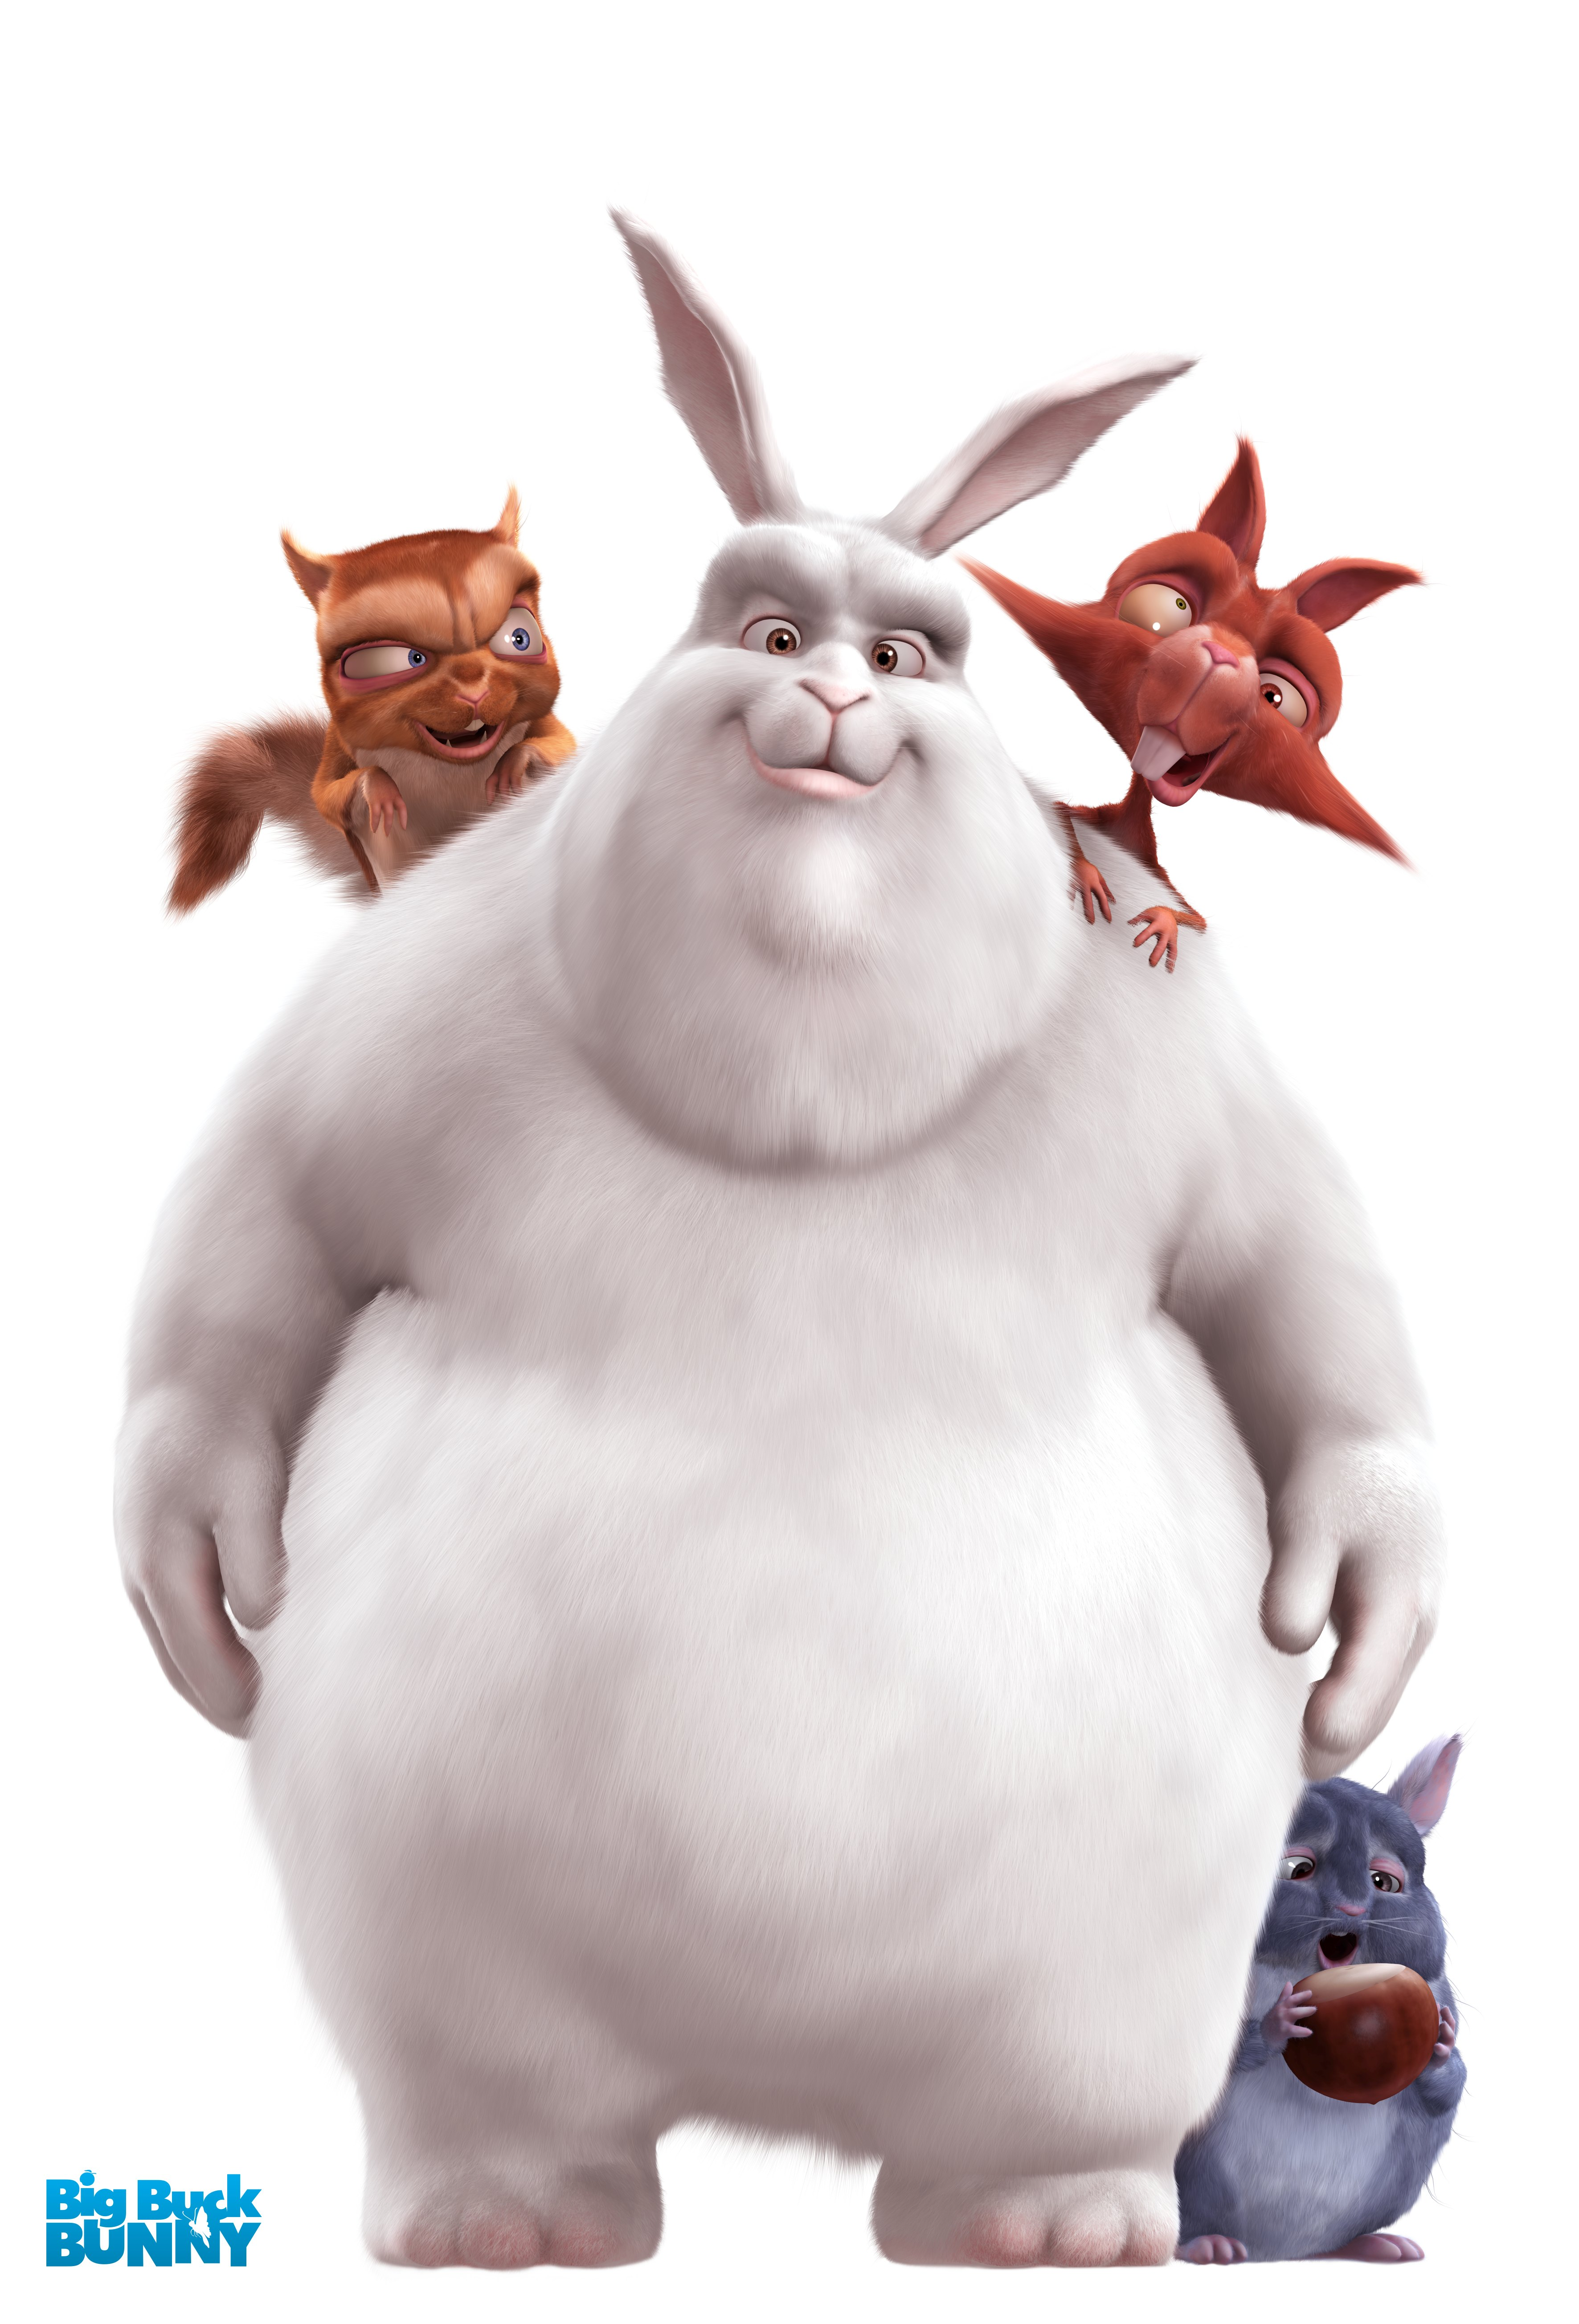
\includegraphics[keepaspectratio,height=5cm]{big_big_buck_bunny.jpg}
\end{figure}

\end{frame}

\section{Interface and modes}

\begin{frame}{Blender interface}

\begin{figure}
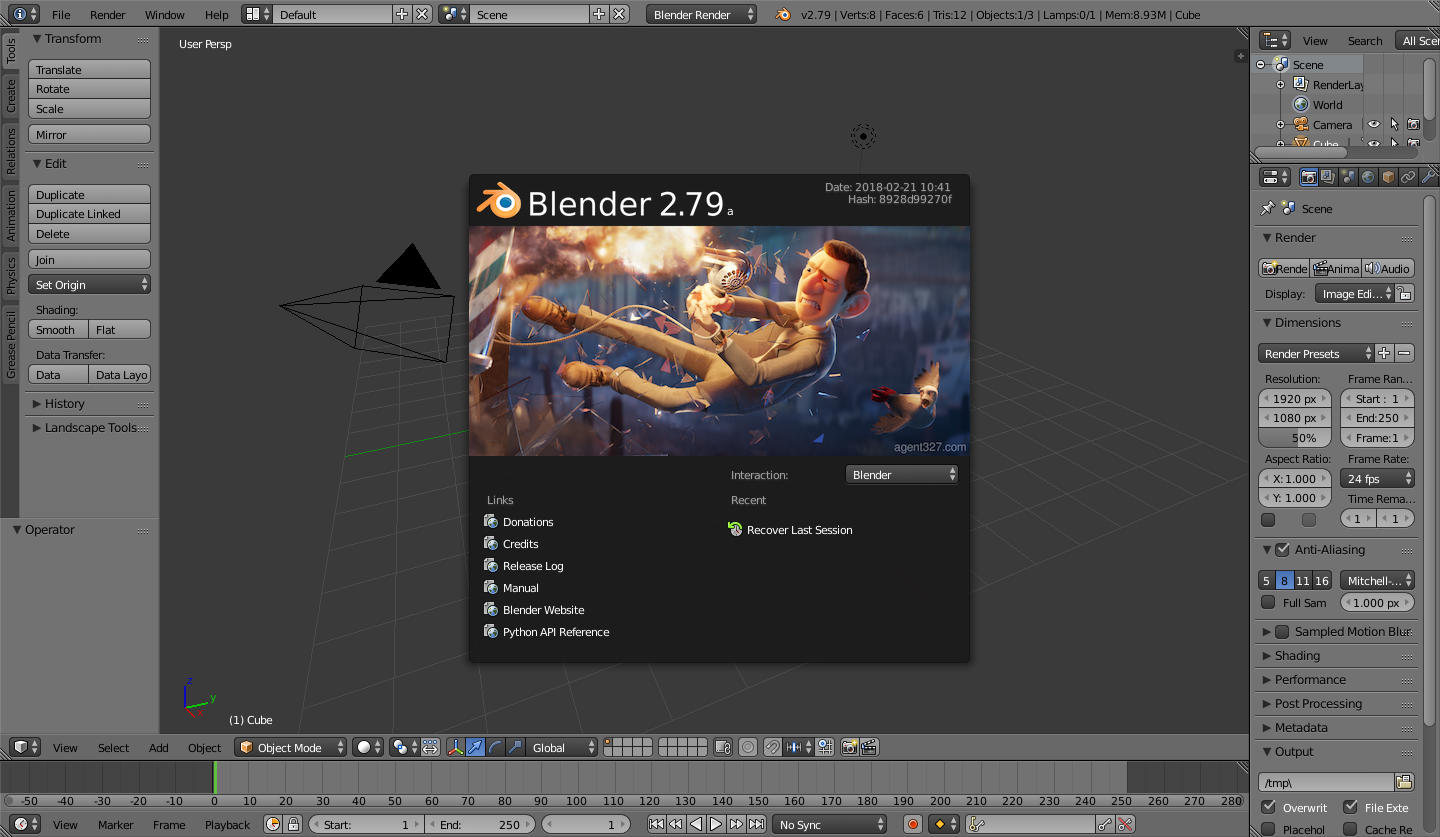
\includegraphics[scale=0.25]{interface.png}
%\caption{Version 2.79, Wikipedia}
\end{figure}

...may be a bit intimidating. We'll go through it in the minute.

\end{frame}

\begin{frame}{Three essential modes}

\begin{itemize}
\item \textbf{Object} - object datablock edition
\item \textbf{Edit} - parts of the mesh (curves and surfaces) edition
\item Sculpt - mesh sculpting (more or less "area-based" mesh edition)
\end{itemize}

\end{frame}

\begin{frame}{First demo}

\centering \Huge
\emph{Let's get familiar with them}

\end{frame}

\section{Shortcuts and editing}

\begin{frame}{How we can edit objects?}
In fact 12 shortcuts + mouse are enough
to do most of the things efficiently. Starting from \textbf{object mode}:
\begin{itemize}
\item \textbf{G}rab
\item \textbf{S}cale
\item \textbf{R}otate
\item \textbf{Shift+A}(dd)
\item \textbf{X} (Cut, of course)
\item Select \textbf{A}ll
\end{itemize}

\end{frame}


\begin{frame}{How we can edit objects?}

...and in edit mode (\textbf{TAB} to switch mode):
\begin{itemize}
\item Add \textbf{F}ace
\item \textbf{E}xtrude
\item \textbf{B} - rectangle selection tool
\item \textbf{C}yclic selection tool
\item \textbf{K}nife
\item \textbf{W} - edit mode popup menu (with operations like Subdivide, Smooth, Bevel and Symmetrize)

\end{itemize}

\end{frame}

\begin{frame}{How we can edit objects?}

\centering \Large
{Beside that, one can also use modifiers available in a separate tab (under shortcuts too): Array, Boolean, Screw and Soldify to name a few}

\end{frame}

\begin{frame}{Second demo}

\centering \Huge
\emph{Back to Blender}

\end{frame}

\section{Rendering}

\begin{frame}{Rendering engines - how to get an image from the scene?}

Short answer: just press \textbf{F12}. There are three rendering engines in 
Blender (you can get more with Add-ons):
\begin{itemize}
\item Blender Render - the oldest and the simplest
\item Blender Game - for the Blender Game Engine; designed for interactive use
\item but all you need is \textbf{Cycles} - physically based 
production renderer for photorealistic images
\end{itemize}

\end{frame}

\begin{frame}{Blender Render vs Cycles Render}

\centering \Huge
...and \textbf{Principled Shader}.

\end{frame}

\begin{frame}{Third demo}

\centering \Huge
\emph{Let's play with Cycles...}

\end{frame}

\section{Learning resources}

\begin{frame}{Learning resources}

\begin{itemize}
\item \href{https://www.blenderguru.com/}{Blender Guru tutorials}
\item \href{https://www.blender.org/support/tutorials/}{Blender.org tutorials}
\item \href{http://polskikursblendera.pl/}{Polski Kurs Blendera}
\end{itemize}

\end{frame}

\begin{frame}{}
  \centering \Huge
  \emph{Questions, comments and feedback}
  
  \centering \Large 
  \href{https://github.com/hryniuk/blender-intro}{github.com/hryniuk/blender-intro}
\end{frame}

\begin{frame}{}
  \centering \Huge
  \emph{Thank You}
  
  \centering \Large
  \href{https://github.com/hryniuk/blender-intro}{github.com/hryniuk/blender-intro}
\end{frame}

\end{document}
